% CFP: https://discourse.llvm.org/t/cfp-llvm-hpc-workshop-at-sc-25/86391
% At least 5 two-column pages, excluding the bibliography and figures

\documentclass[acmtog,natbib=false]{acmart}
\AtBeginDocument{\providecommand\BibTeX{{ Bib\TeX}}}

\RequirePackage[
datamodel=acmdatamodel,
style=acmnumeric, % use style=acmauthoryear for publications that require it
]{biblatex}
\addbibresource{references.bib}

\usepackage[T1]{fontenc}
\usepackage{listings}
\usepackage{xspace}
\usepackage[printonlyused]{acronym}

%% Rights management information.  This information is sent to you
%% when you complete the rights form.  These commands have SAMPLE
%% values in them; it is your responsibility as an author to replace
%% the commands and values with those provided to you when you
%% complete the rights form.
\setcopyright{acmlicensed}
\copyrightyear{2025}
\acmYear{2025}
\acmDOI{XXXXXXX.XXXXXXX}

%%
%% Submission ID.
%% Use this when submitting an article to a sponsored event. You'll
%% receive a unique submission ID from the organizers
%% of the event, and this ID should be used as the parameter to this command.
\acmSubmissionID{tbd}

%% configure the listings package
\lstset{
  basicstyle=\ttfamily\small,
  captionpos=b,
}

%% useful macros
\newcommand{\todo}[1]{\textcolor{red}{#1}}
\newcommand{\code}[1]{\texttt{#1}\xspace}
\newcommand{\registered}[0]{\textsuperscript{\textregistered}\xspace}
\newcommand{\trademark}[0]{\texttrademark\xspace}

\begin{document}
\title{Implementing OpenMP\registered Offload Support in LLVM Flang}

\author{Dominik Adamski}
\email{dominik.adamski@amd.com}
\orcid{}
\affiliation{%
  \institution{Advanced Micro Devices}
  \city{tbd}
  \state{tbd}
  \country{Poland}
}

\author{Michael Klemm}
\email{michael.klemm@amd.com}
\orcid{0000-0002-8634-4634}
\affiliation{%
  \institution{Advanced Micro Devices GmbH}
  \city{Munich}
  \state{BY}
  \country{Germany}
}

\author{Andrew Gozillon}
\email{andrew.gozillon@amd.com}
\orcid{0000-0001-7558-7166}
\affiliation{%
  \institution{Advanced Micro Devices AB}
  \city{Malmo}
  \state{Skåne County}
  \country{Sweden}
}

\renewcommand{\shortauthors}{Adamski et al.}

\begin{abstract}
Lorem ipsum dolor sit amet, consectetur adipisicing elit, sed do eiusmod
tempor incididunt ut labore et dolore magna aliqua. Ut enim ad minim veniam,
quis nostrud exercitation ullamco laboris nisi ut aliquip ex ea commodo
consequat. Duis aute irure dolor in reprehenderit in voluptate velit esse
cillum dolore eu fugiat nulla pariatur. Excepteur sint occaecat cupidatat non
proident, sunt in culpa qui officia deserunt mollit anim id est laborum.
Lorem ipsum dolor sit amet, consectetur adipisicing elit, sed do eiusmod
tempor incididunt ut labore et dolore magna aliqua. Ut enim ad minim veniam,
quis nostrud exercitation ullamco laboris nisi ut aliquip ex ea commodo
consequat. Duis aute irure dolor in reprehenderit in voluptate velit esse
cillum dolore eu fugiat nulla pariatur. Excepteur sint occaecat cupidatat non
proident, sunt in culpa qui officia deserunt mollit anim id est laborum.
\end{abstract}

%% generate via: https://dl.acm.org/ccs
\begin{CCSXML}
<ccs2012>
   <concept>
       <concept_id>10011007.10011006.10011041</concept_id>
       <concept_desc>Software and its engineering~Compilers</concept_desc>
       <concept_significance>500</concept_significance>
       </concept>
   <concept>
       <concept_id>10010147.10010169.10010175</concept_id>
       <concept_desc>Computing methodologies~Parallel programming languages</concept_desc>
       <concept_significance>500</concept_significance>
       </concept>
   <concept>
       <concept_id>10010520.10010521.10010542.10010546</concept_id>
       <concept_desc>Computer systems organization~Heterogeneous (hybrid) systems</concept_desc>
       <concept_significance>500</concept_significance>
       </concept>
 </ccs2012>
\end{CCSXML}
\ccsdesc[500]{Software and its engineering~Compilers}
\ccsdesc[500]{Computing methodologies~Parallel programming languages}
\ccsdesc[500]{Computer systems organization~Heterogeneous (hybrid) systems}

\keywords{LLVM, Flang, OpenMP, GPU, Accelerators}

\received{20 February 2007}
\received[revised]{12 March 2009}
\received[accepted]{5 June 2009}

\maketitle

\section{Introduction}
\label{sec:Introduction}
\Ac{GPU} is an acronym, and let's use a citation~\cite{AMD24}.

\section{LLVM Flang Compiler}
\label{sec:LLVMFlangCompiler}

\subsection{Fortran Compiler Pipeline}
\label{sec:FortranCompilerPipeline}
\todo{This is a copy of another paper; this needs to be reworded and extended.}

\begin{figure}[t]
\centering
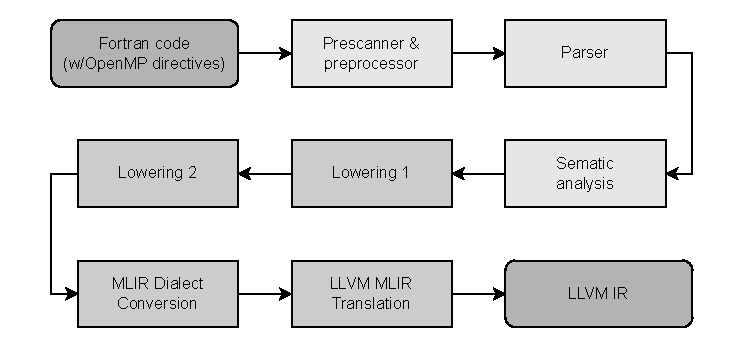
\includegraphics[width=\linewidth]{figures/flang_compiler_phases_overview.pdf}
\caption{Simplified overview of the compiler phases in the AMD Next-Gen Fortran Compiler front-end.\label{fig:FlangCompilerPhases}}
\end{figure}

\begin{figure}[t]
\lstinputlisting[language=Fortran,
                caption={Example Fortran code with \code{!\$omp target team loop} construct and \code{map} clauses},
                label={lst:FortranExample}]
                {code/tgt_loop.f90}
\end{figure}

\begin{figure}[t]
\lstinputlisting[language=Fortran,
                caption={Fortran code of Listing~\ref{lst:FortranExample} after preprocessing and prescanning.},
                label={lst:FortranExampleCooked}]
                {code/tgt_loop_cooked.f90}
\end{figure}

Figure~\ref{fig:FlangCompilerPhases} shows a simplified overview of the compiler pipeline of the LLVM Flang compiler frontend up to LLVM \ac{IR} generation.
The same stages are also used by the AMD Next-Gen Fortran Compiler front-end.
In the Prescanner \& Preprocessor stage, the lexical analysis and C-style processor produce a stream of characters of normalized Fortran source code (see Listing~\ref{lst:NormalizedFortranCooked}). 
This code contains expanded preprocessor macros, included code resulting from \code{INCLUDE} statements, and removed unnecessary blank characters and comments.
Compiler directives such as \code{!\$dir} and the OpenMP directives introduced with \code{!\$omp} remain in the stream of characters.
The parser and semantic analysis stages then construct a parse tree of the processed Fortran code and annotate it with semantic information (e.g., data types).
The parse tree contains all details about OpenMP directives, clauses, etc. as nodes in the tree.

The parse tree is then gradually lowered into different levels of intermediate representation, depending on the needs of the applied transformation and optimization passes.
First, the parse tree and the contained OpenMP directive structure are transformed into \ac{HLFIR} and \ac{FIR}, both of which are based on \ac{MLIR}.
\Ac{HLFIR} provides additional high-level information over \ac{FIR} about the specific semantics of Fortran (e.g., array operations that can be used to optimize Fortran array statements).
It also has additional information in the type system to represent Fortran attributes for (dummy) variables.
Both \ac{HLFIR} and \ac{FIR} still contain explicit information about the OpenMP directives and clauses as well as their nesting structure.
For instance, \code{DO} loop nest is associated with the corresponding OpenMP \code{target teams loop} construct (see Figure~\ref{fig:MLIROffloadIR}\todo{Add example of a simple offload region and show MLIR for it.})
Finally, the \ac{MLIR} code is transformed into regular LLVM \ac{IR} and is passed to the compiler back-end for target code generation.


\subsection{OpenMP Code Generation}
\label{sec:OpenMPCodeGen}

During lowering, the compiler outlines OpenMP \code{target} regions and creates kernel functions per region such that the back-end can generate \ac{GPU} code for those in addition to host code.
The original intermediate code is then replaced with boilerplate code to launch the created kernel functions.
This involves generated code to perform data mapping according to the OpenMP semantics and code to invoke the kernel on the GPU via the runtime libraries.

\todo{Andrew: you could write about the actual lowering and code-gen for OpenMP, focus on GPU code-gen and outlining.}



\section{Conclusions}
\label{sec:Conclusions}

\section*{List of Acronyms}

\begin{acronym}[paper]
\acro{AST}[AST]{Abstract Syntax Tree}
\acro{API}[API]{application programming interface}
\acro{CCD}[CCD]{compute complex die}
\acro{CFD}[CFD]{computational fluid dynamics}
\acro{CU}[CU]{compute unit}
\acro{FIR}[FIR]{Fortran intermediate representation}
\acro{GPU}[GPU]{graphics processing unit}
\acro{HLFIR}[HLFIR]{high-level Fortran intermediate representation}
\acro{HPC}[HPC]{high-performance computing}
\acro{IPO}[IPO]{interprocedural optimization}
\acro{IR}[IR]{intermediate representation}
\acro{LTO}[LTO]{link time optimization}
\acro{MLIR}[MLIR]{multi-level intermediate representation}
\acro{XCD}[XCD]{accelerator complex die}
\acro{WENO}[WENO]{weighted essentially non-oscillatory}
\acro{SDK}[SDK]{software development kit}
\acro{HIP}[HIP]{Heterogeneous-computing Interface for Portability}
\acro{IFA}[IFA]{isolated from above}
\acro{PFT}[PFT]{Pre-FIR Tree}
\acro{RTL}[RTL]{run-time library}
\end{acronym}

\section*{Acknowledgments}
Copyright 2025 Advanced Micro Devices, Inc.
AMD, the AMD Arrow logo, Instinct, Radeon, and EPYC, and combinations thereof are trademarks of Advanced Micro Devices, Inc.
Other product names used in this publication are for identification purposes only and may be trademarks of their respective companies.

\printbibliography

\end{document}
